% \begin{figure}[hpbt!]
% 	\begin{center}
% 		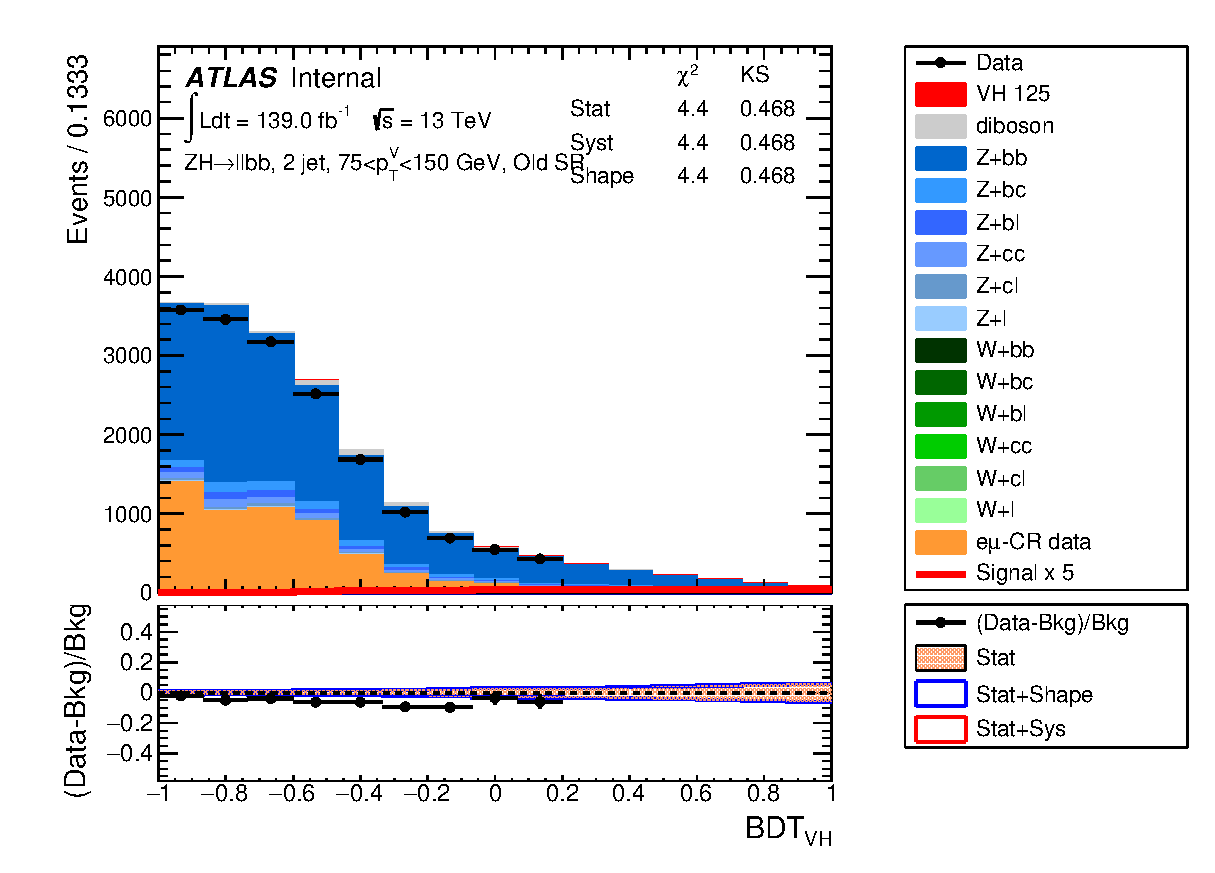
\includegraphics[width=75mm]{\ddtt@figures/dataMC_ade/C_2tag2jet_75_150ptv_SROld_mva_trafo.eps}
% 		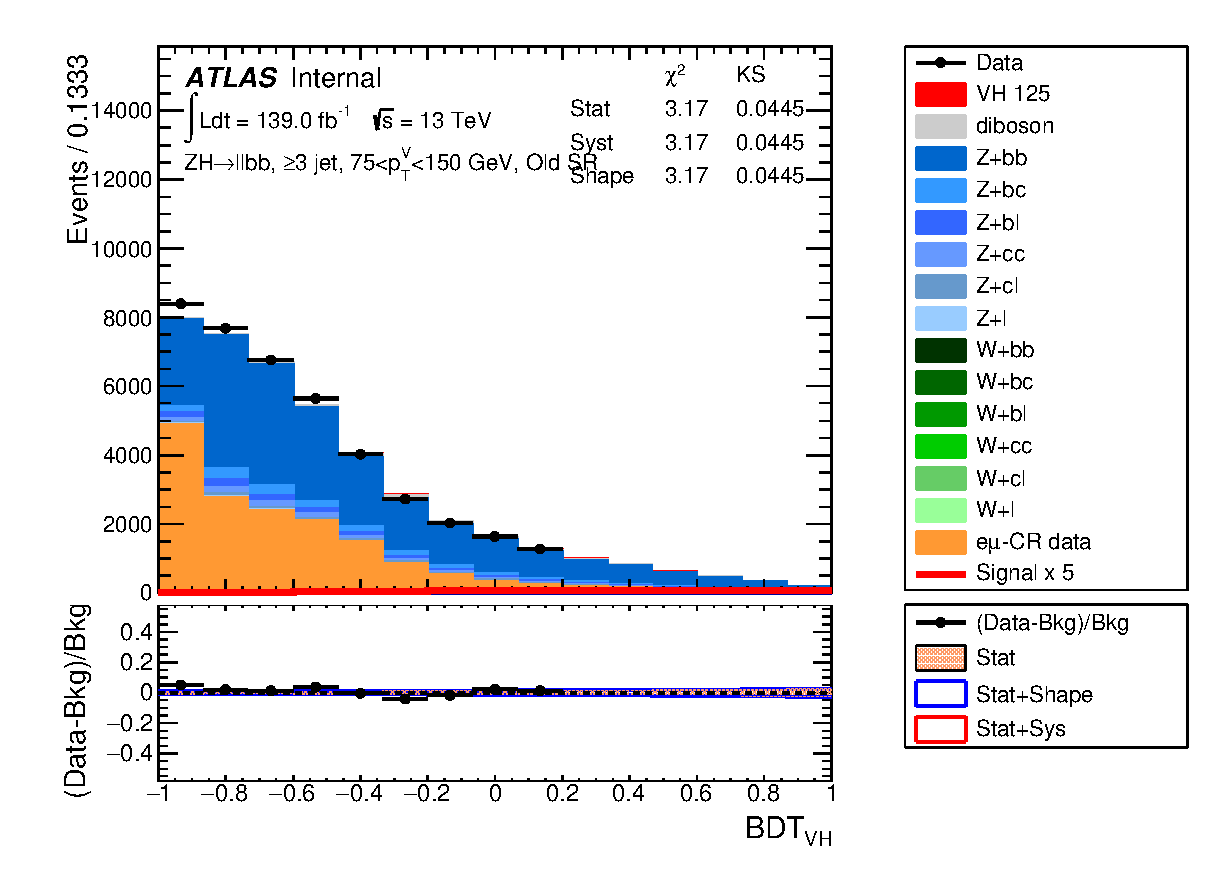
\includegraphics[width=75mm]{\ddtt@figures/dataMC_ade/C_2tag3pjet_75_150ptv_SROld_mva_trafo.eps}
% 		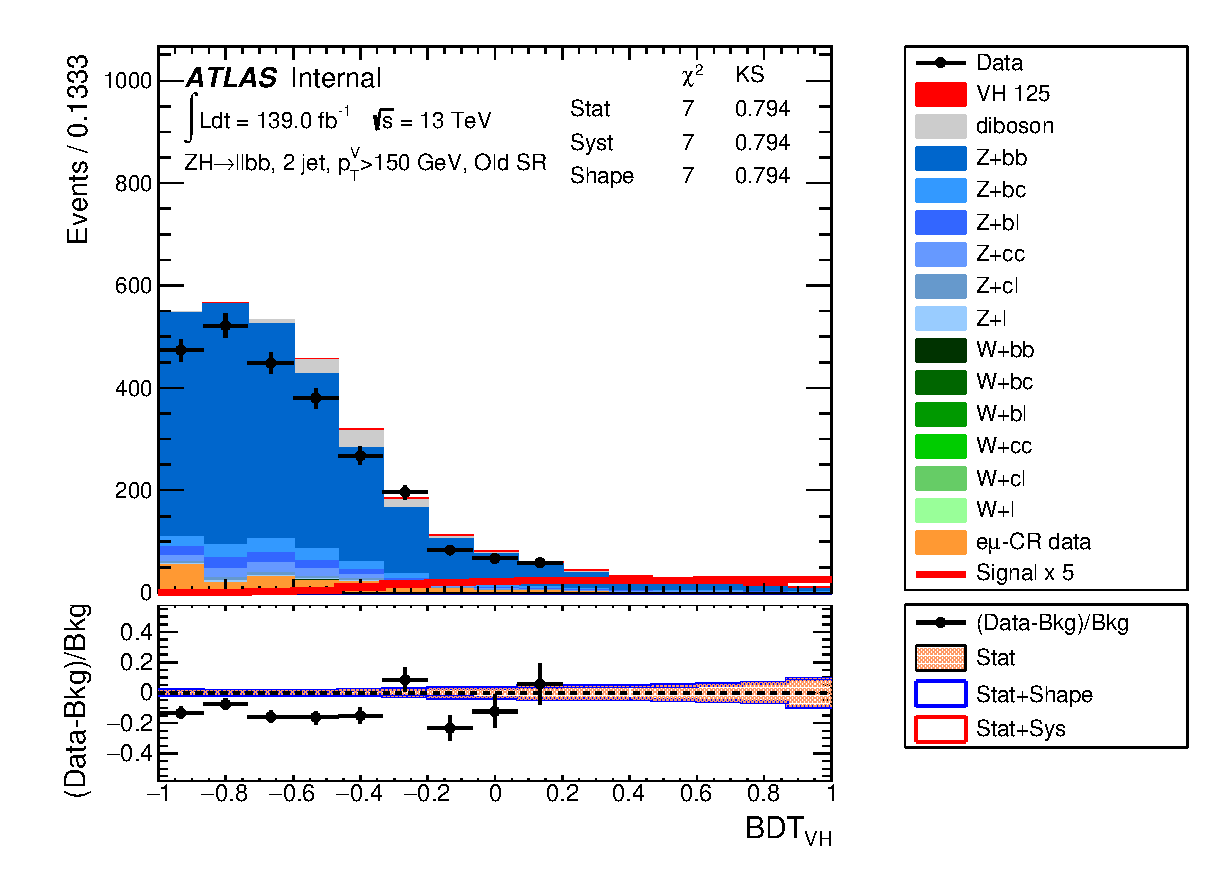
\includegraphics[width=75mm]{\ddtt@figures/dataMC_ade/C_2tag2jet_150ptv_SROld_mva_trafo.eps}
% 		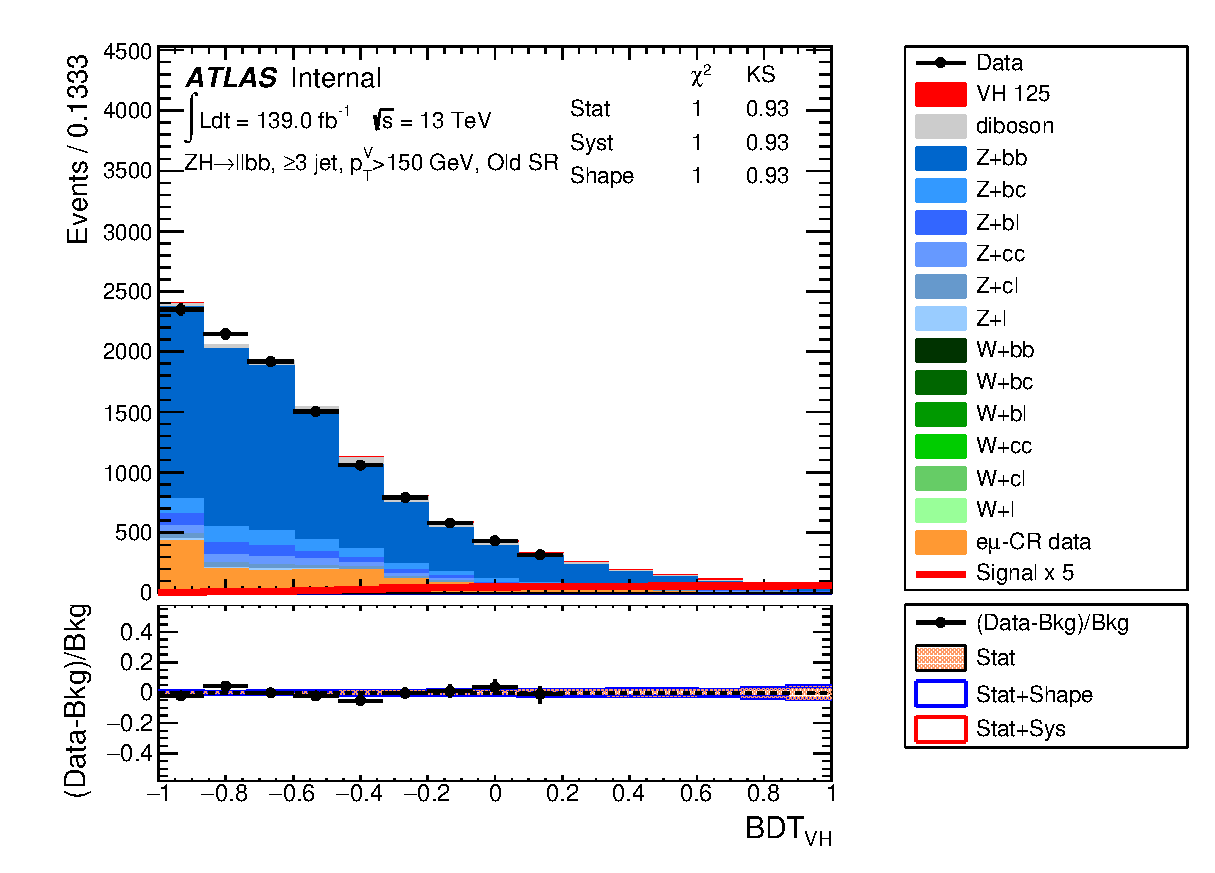
\includegraphics[width=75mm]{\ddtt@figures/dataMC_ade/C_2tag3pjet_150ptv_SROld_mva_trafo.eps}				
% 	\end{center}
% 	\caption{Data-MC comparison of BDT output distributions in SR in each \ptv{} and nJet bin.}
% 	\label{fig:DataMCmva}
% \end{figure}
\begin{figure}[hpbt!]
	\centering
  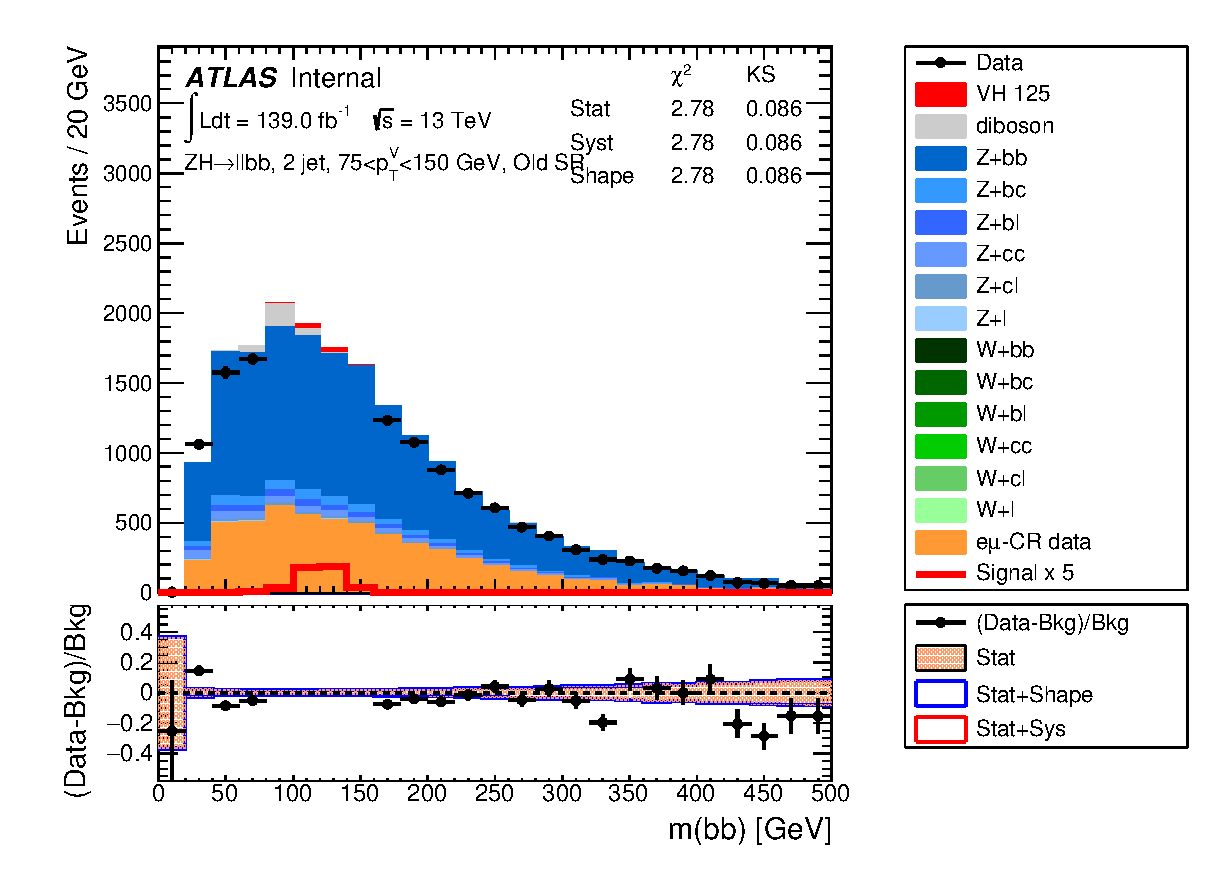
\includegraphics[width=75mm]{dataMC_ade/C_2tag2jet_75_150ptv_SROld_mBB.eps}
  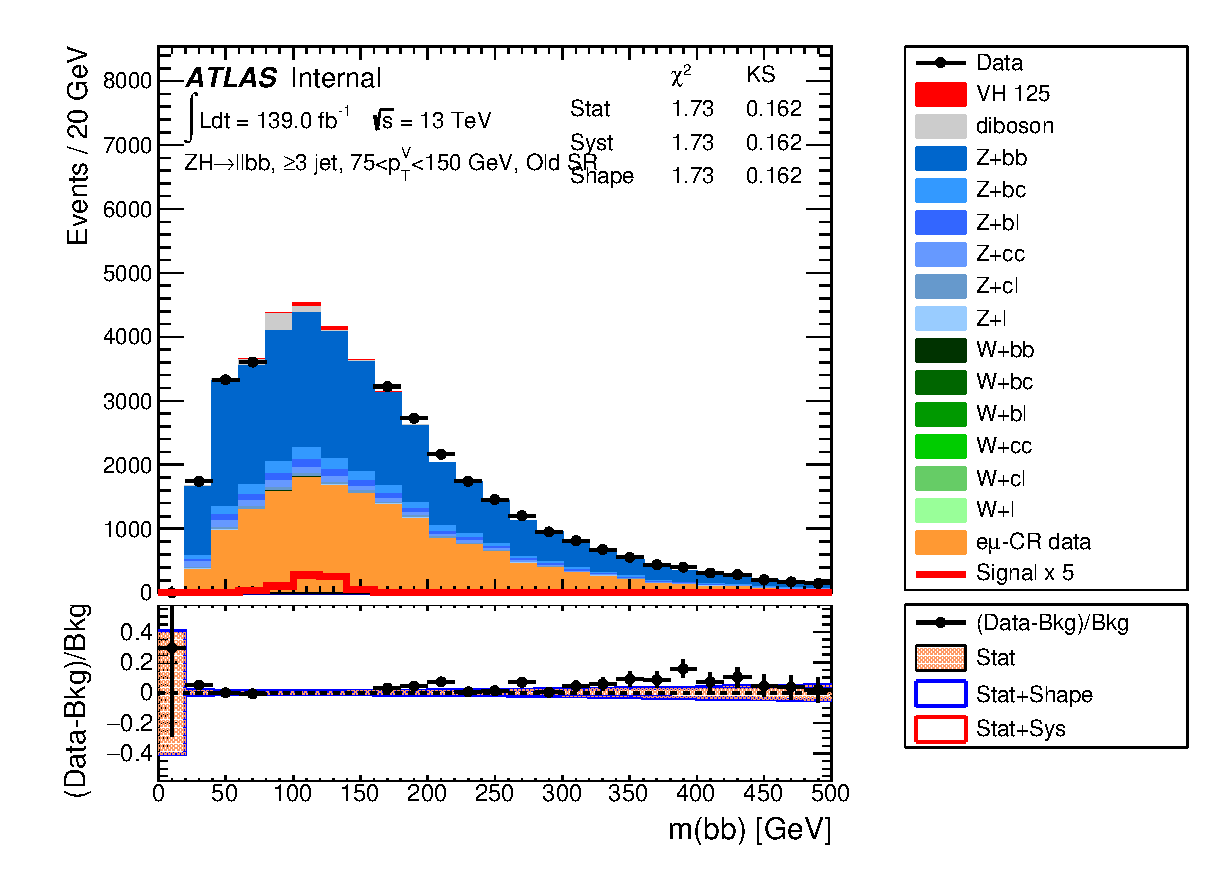
\includegraphics[width=75mm]{C_2tag3pjet_75_150ptv_SROld_mBB.eps}
  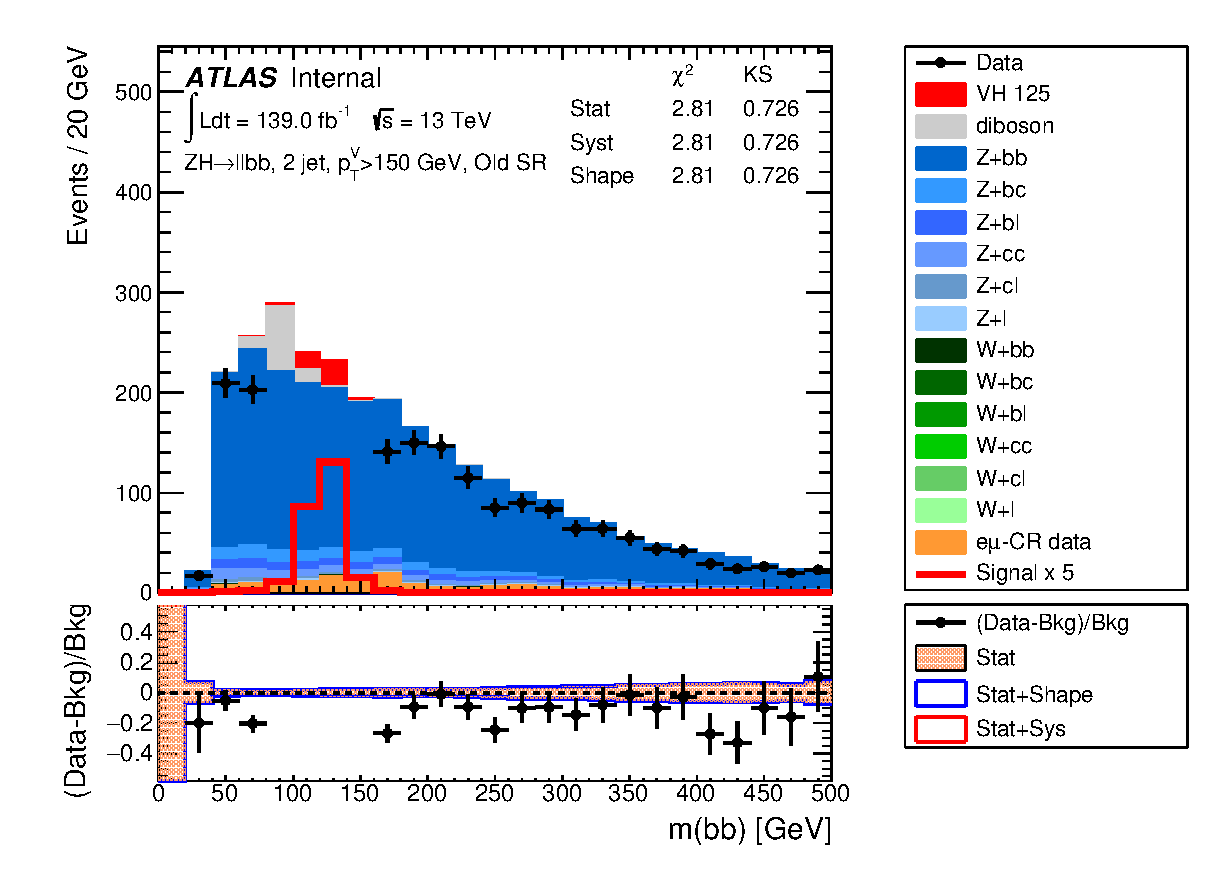
\includegraphics[width=75mm]{C_2tag2jet_150ptv_SROld_mBB.eps}
  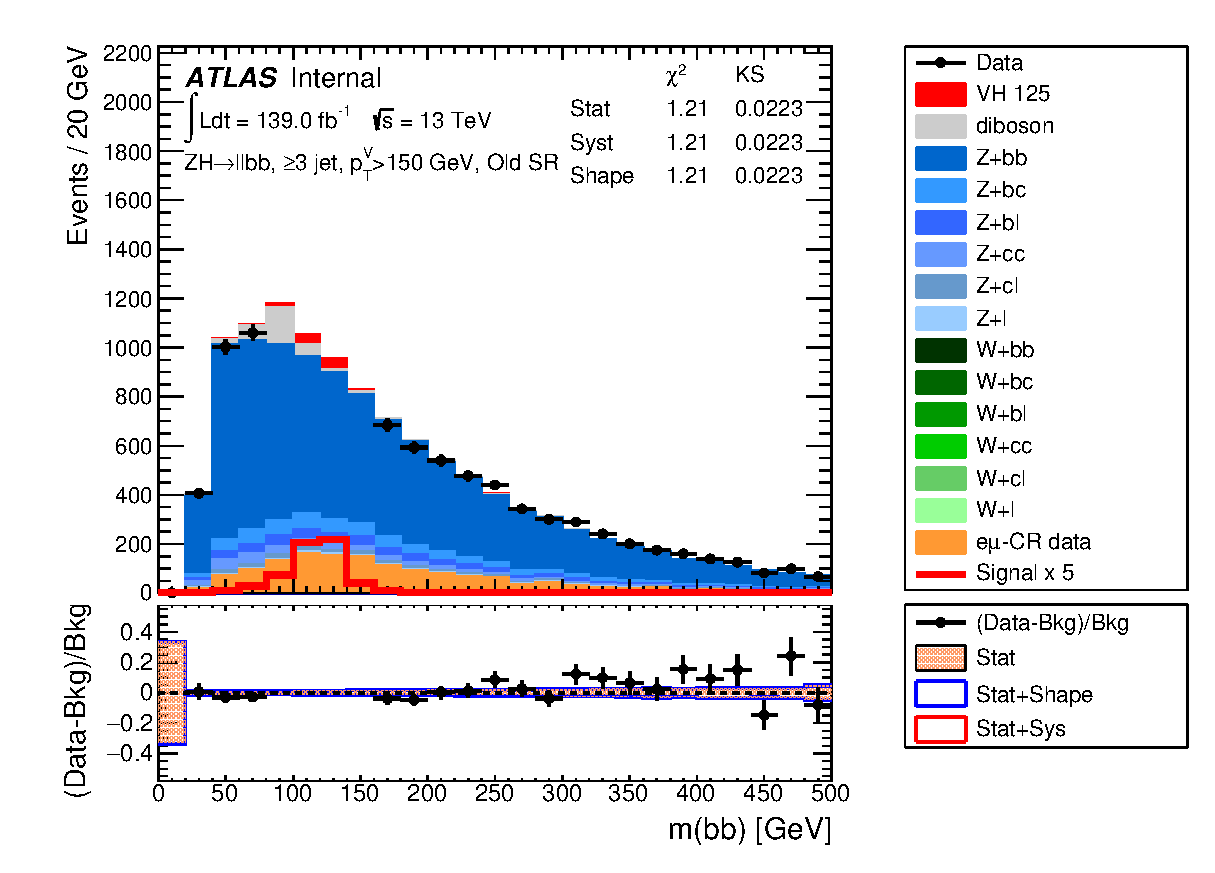
\includegraphics[width=75mm]{dataMC_ade/C_2tag3pjet_150ptv_SROld_mBB.eps}				
	\caption{Data versus prediction comparison of $m_{bb}$ distributions used to
    check how well the top $e\mu$ control region data models the shape of the
    $t\bar{t}$ and single top processes.}
	\label{fig:ttbardd-mbb}
\end{figure}
% \newcommand{\figDataMCptv}{
% \begin{figure}[bt]
% 	\begin{center}
% 		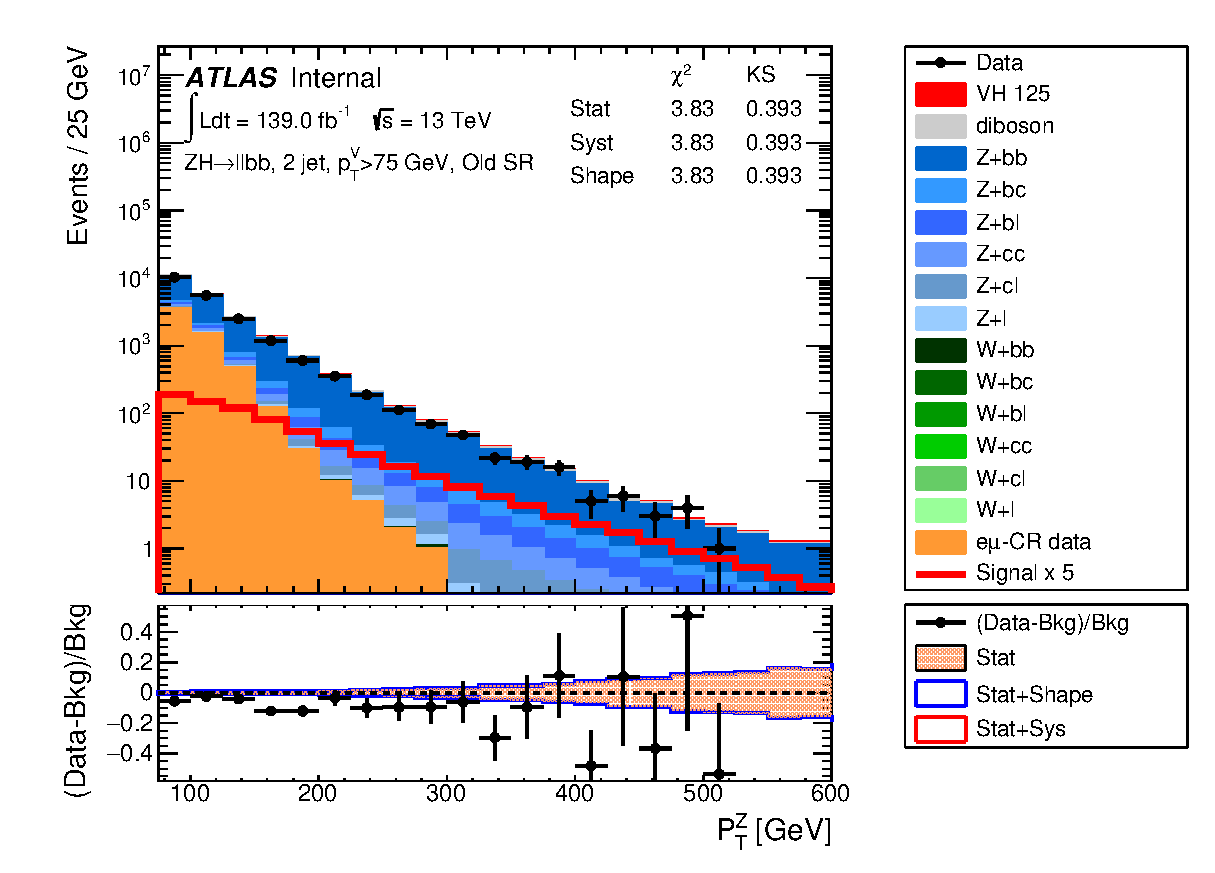
\includegraphics[width=75mm]{\ddtt@figures/dataMC_ade/C_2tag2jet_75ptv_SROld_pTV_Log.eps}
% 		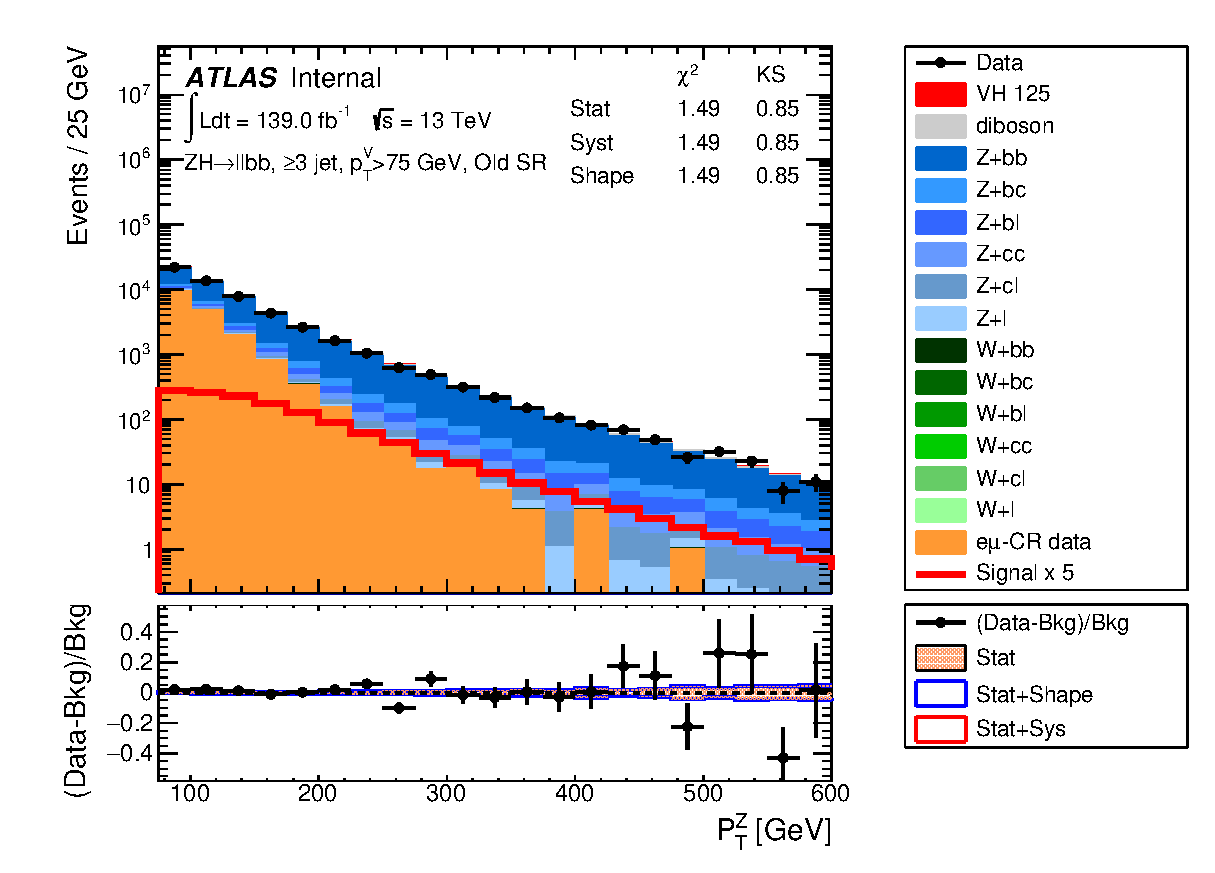
\includegraphics[width=75mm]{\ddtt@figures/dataMC_ade/C_2tag3pjet_75ptv_SROld_pTV_Log.eps}
% 	\end{center}
% 	\caption{Data-MC comparison of $p_{{\textrm T},V}$ distributions in SR in each nJet bin.}
% 	\label{fig:DataMCptv}
% \end{figure}
% }
% \newcommand{\figDataMCnjet}{
% \begin{figure}[bt]
% 	\begin{center}
% 		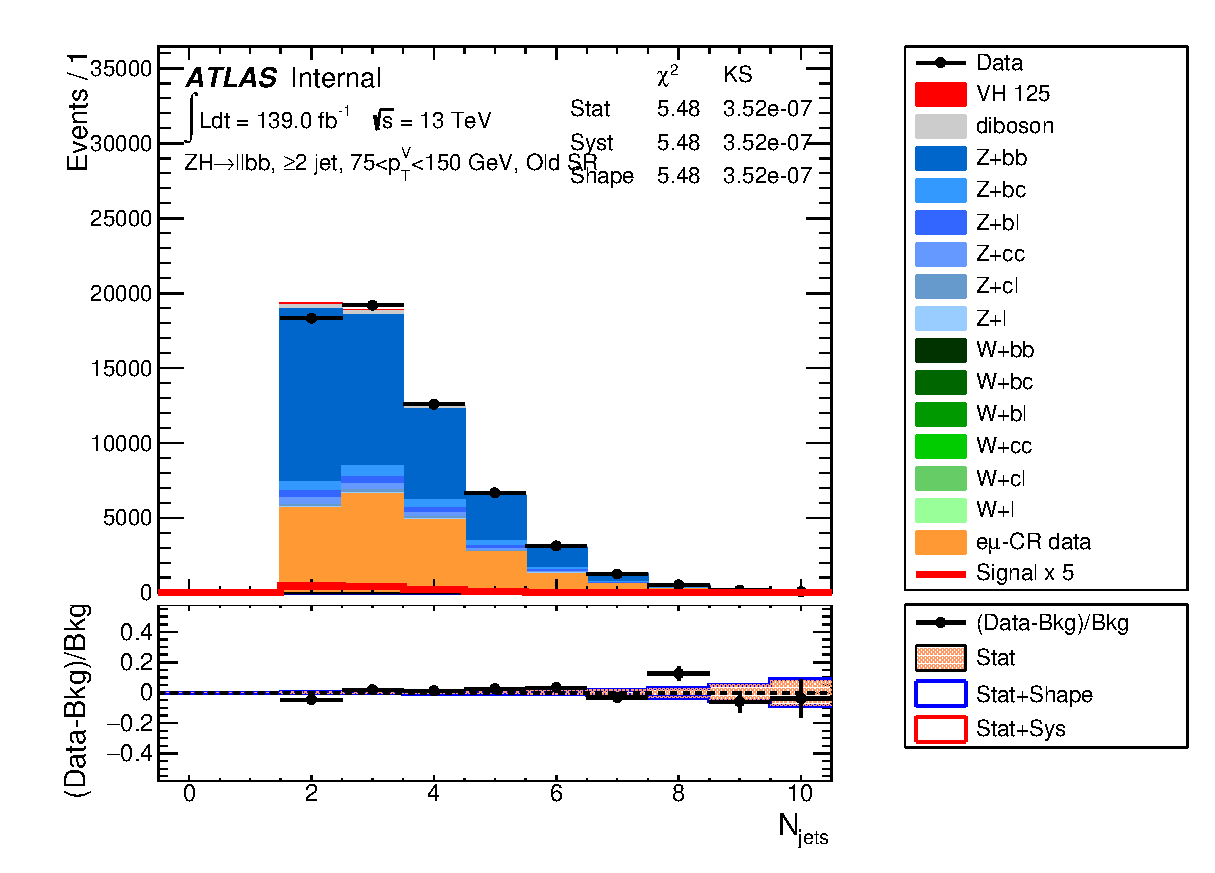
\includegraphics[width=75mm]{\ddtt@figures/dataMC_ade/C_2tag2pjet_75_150ptv_SROld_NJets.eps}
% 		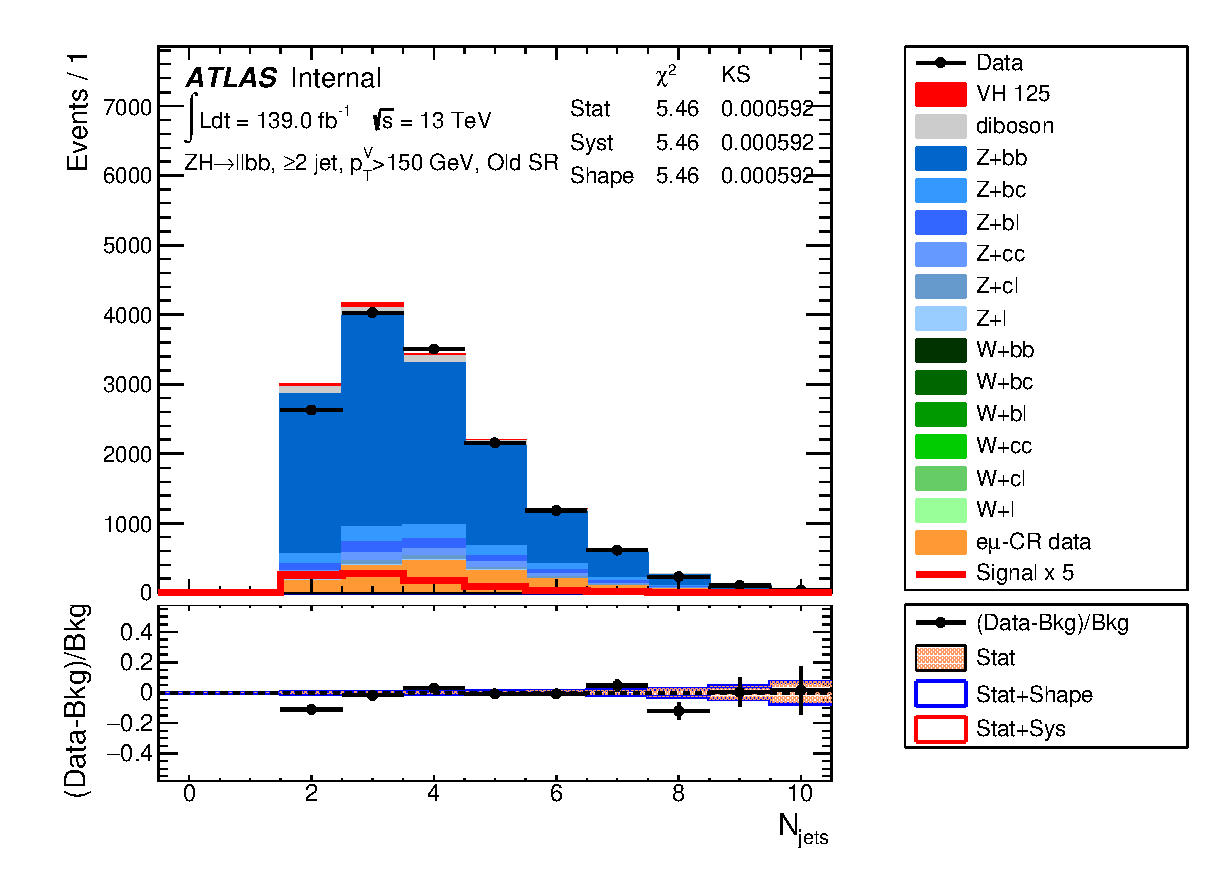
\includegraphics[width=75mm]{\ddtt@figures/dataMC_ade/C_2tag2pjet_150ptv_SROld_NJets.eps}
% 	\end{center}
% 	\caption{Data-MC comparison of nJets distributions in SR in each $p_{{\textrm T},V}$ bin.}
% 	\label{fig:DataMCnjet}
% \end{figure}
% }